\subsubsection{Phát biểu bài toán LDA tổng quát}  

Cho tập dữ liệu gồm \( N \) điểm \( \mathbf{x}_1, \mathbf{x}_2, ..., \mathbf{x}_N \) trong không gian \( d \)-chiều.  
Các điểm dữ liệu được chia thành \( K \) lớp, với mỗi lớp \( k \) chứa \( N_k \) điểm.  
Ký hiệu tập chỉ số của lớp \( k \) là:  
\[
\mathbf{C}_k = \{ n \; | \; n \in \text{lớp } k \}, \quad k = 1,2,...,K.
\]  
\textbf{Đầu ra}  

Ma trận chiếu \( W \in \mathbb{R}^{d \times (K-1)} \), trong đó mỗi cột là một vector chiếu \( \mathbf{w}_i \).  
Dữ liệu sau khi chiếu xuống không gian mới:  
\[
\mathbf{y}_n = W^T \mathbf{x}_n, \quad 1 \leq n \leq N.
\]  
Với \( \mathbf{y}_n \) thuộc không gian \( (K-1) \)-chiều  sao cho các điểm dữ liệu thuộc các lớp khác nhau được phân tách tốt nhất trong không gian mới này.

 
\subsubsection{Ý tưởng giải quyết bài toán}  

Để tiếp cận bài toán phân lớp nhiều lớp, trước hết xem xét bài toán đơn giản nhất: phân loại hai lớp.  

\textbf{Bài toán LDA hai lớp}  

Xét bài toán phân loại hai lớp (lớp \( C_1 \) - màu đỏ và lớp \( C_2 \) - màu xanh).  

\begin{figure}[htbp]
    \centering
    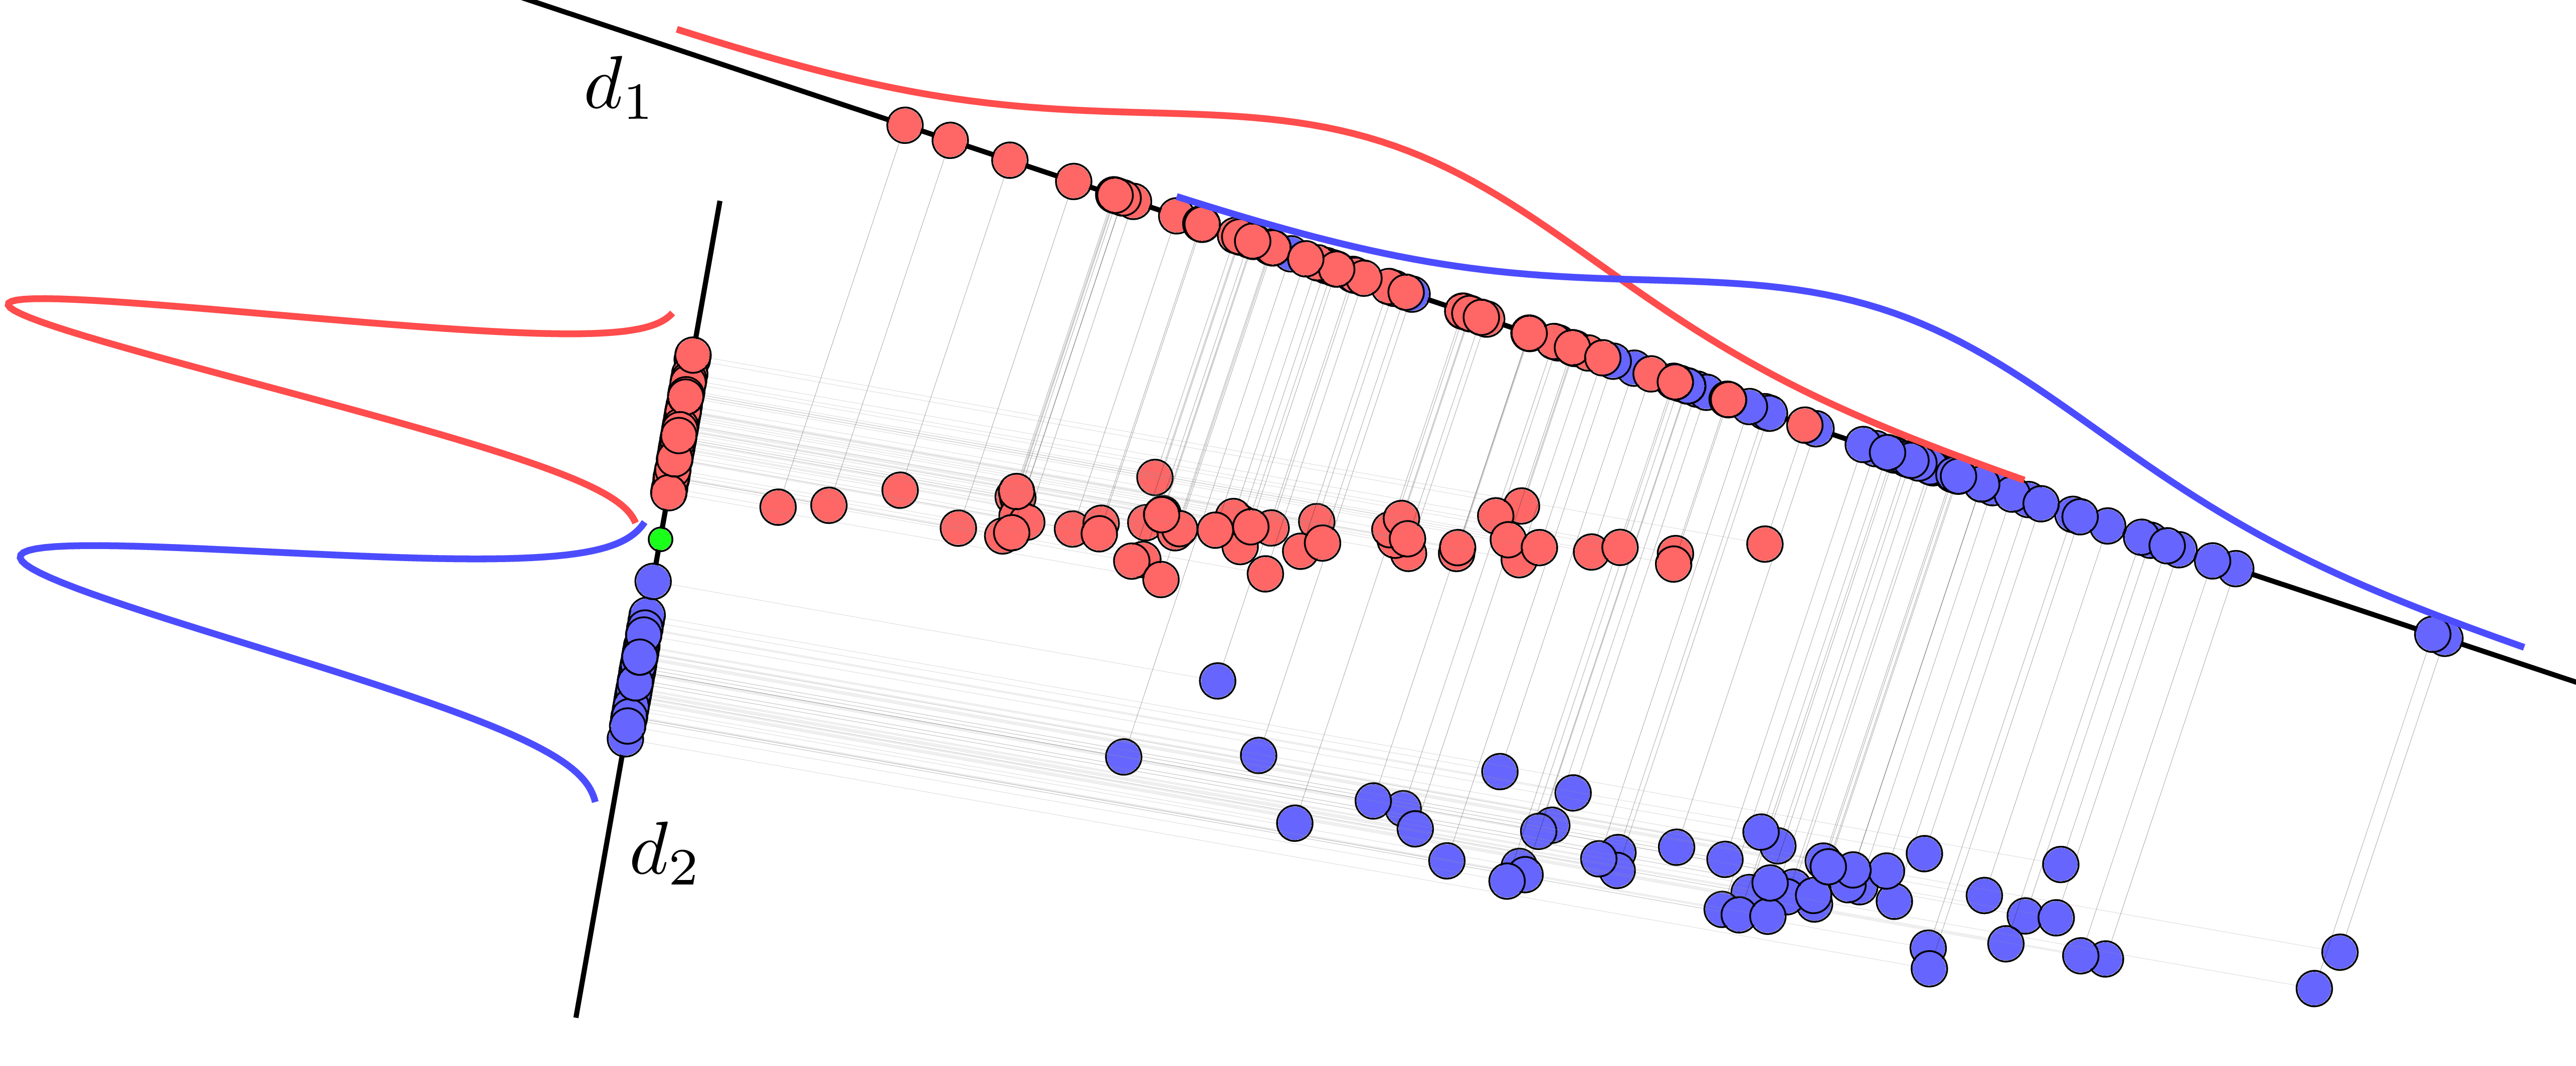
\includegraphics[width=0.6\textwidth]{assets/2_1_1.png}
    \caption{Trực quan hóa dữ liệu }
    \label{fig:example}
\end{figure}
  
\textbf{Giả sử:}  
\begin{itemize}
    \item Dữ liệu của hai lớp có phân phối chuẩn.  
    \item Giá trị kỳ vọng của mỗi lớp lần lượt là \( \mathbf{m}_1 \) và \( \mathbf{m}_2 \). 
    \item Độ phân tán của dữ liệu trong từng lớp được đo bằng phương sai \( s_1^2 \) và \( s_2^2 \).
\end{itemize}

\textbf{Bài toán đưa về thành:} Tìm một hướng chiếu \( \mathbf{w} \) sao cho dữ liệu của hai lớp tách biệt rõ ràng nhất.

Trước khi tìm lời giải, ta xét các trường hợp về cách dữ liệu bị phân tán khi chiếu lên một trục bất kỳ.  

\hspace{1cm}\textbf{Trường hợp 1: Hai lớp dữ liệu có phương sai lớn}  

\begin{figure}[htbp]
    \centering
    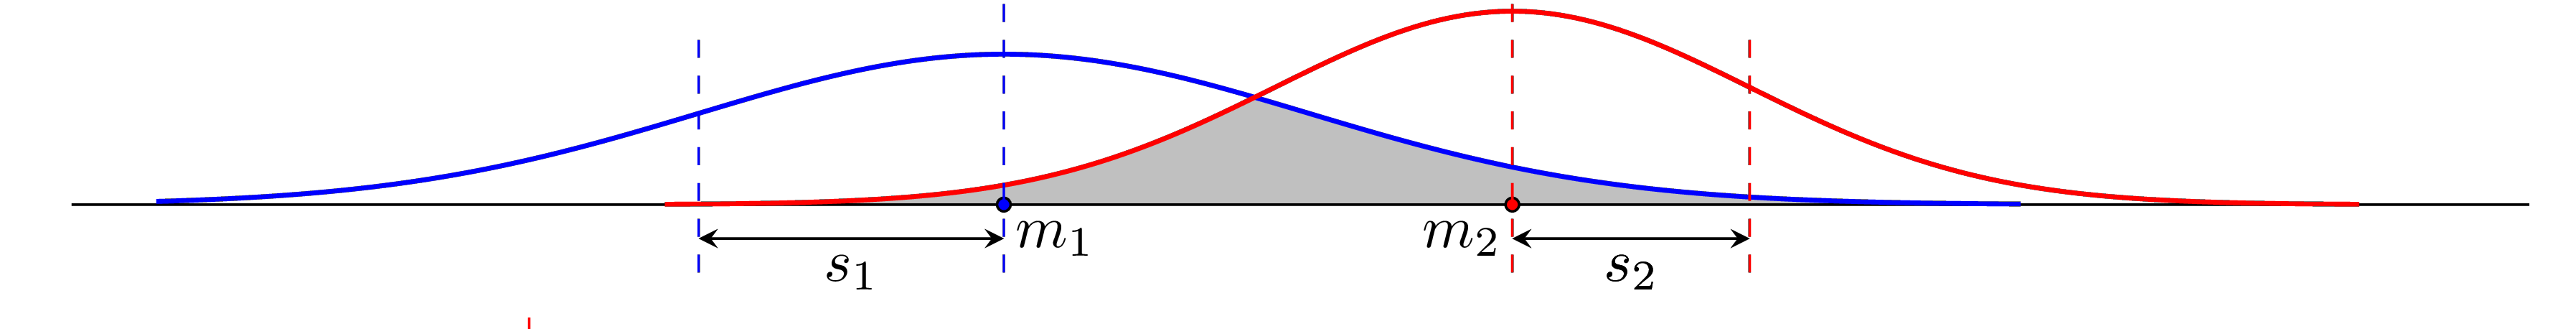
\includegraphics[width=0.9\textwidth]{assets/2_1_1a.png}
    \caption{Trường hợp 1: Phương sai lớn làm dữ liệu chồng lấn nhiều}
    \label{fig:case1}
\end{figure}

\hspace{1cm}Khi dữ liệu trong mỗi lớp có phương sai lớn, các điểm dữ liệu bị trải rộng và có phần chồng lấn lớn.  

\hspace{1cm}\textbf{Trường hợp 2: Phương sai nhỏ nhưng khoảng cách giữa trung tâm hai lớp quá gần}  

\begin{figure}[htbp]
    \centering
    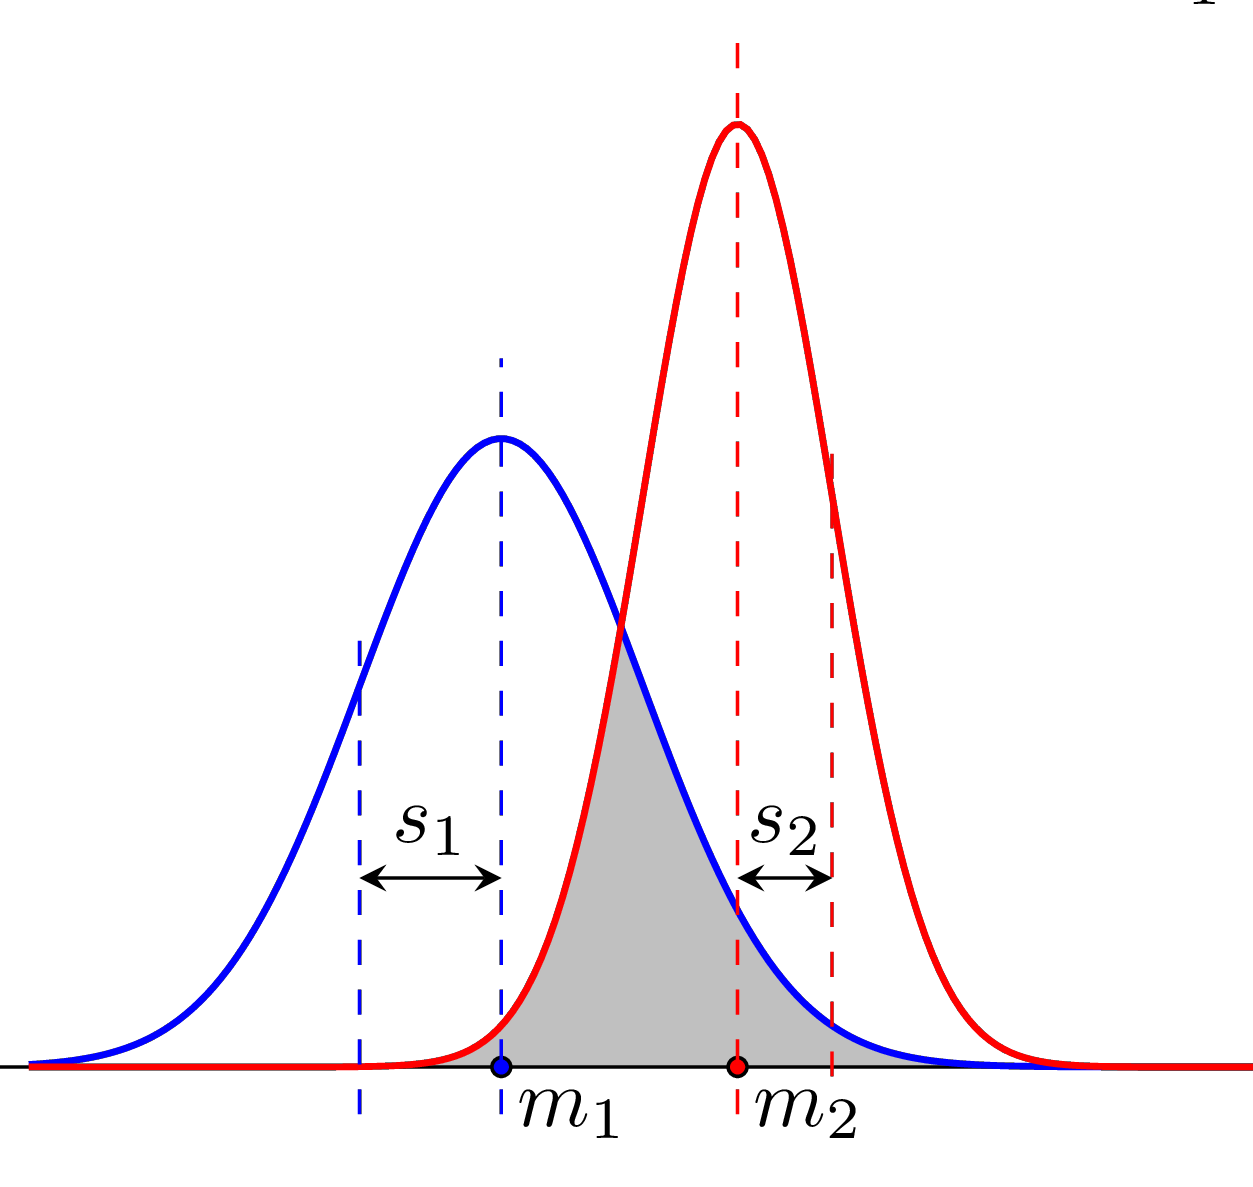
\includegraphics[width=0.3\textwidth]{assets/2_1_1b.png}
    \caption{Trường hợp 2: Trung tâm hai lớp quá gần nhau}
    \label{fig:case2}
\end{figure}

\hspace{1cm}Khi phương sai nhỏ, dữ liệu trong từng lớp ít phân tán, nhưng nếu trung tâm hai lớp \( \mathbf{m}_1 \) và \( \mathbf{m}_2 \) gần nhau, phần chồng lấn giữa hai lớp vẫn lớn.  

\hspace{1cm}\textbf{Trường hợp 3: Phương sai nhỏ và khoảng cách giữa hai trung tâm đủ lớn}  

\begin{figure}[htbp]
    \centering
    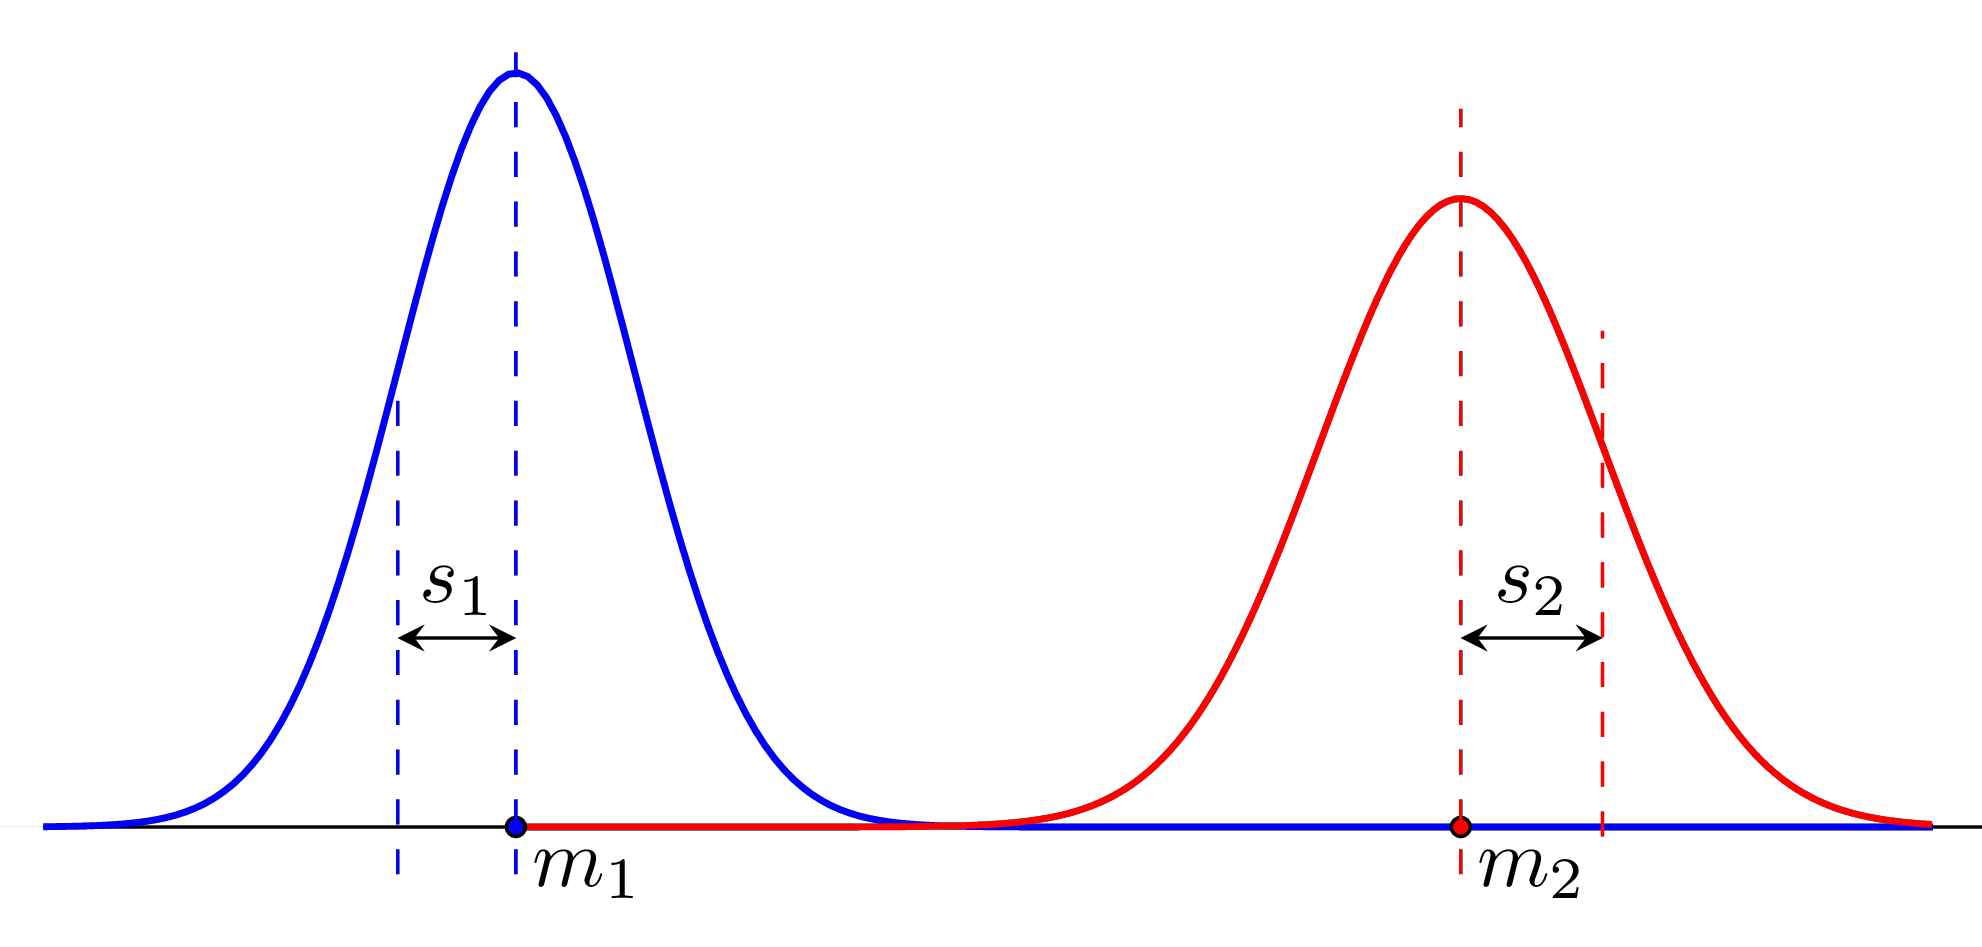
\includegraphics[width=0.5\textwidth]{assets/2_1_1c.png}
    \caption{Trường hợp 3: Phân bố tốt nhất để phân lớp}
    \label{fig:case3}
\end{figure}

\hspace{1cm}Khi dữ liệu trong mỗi lớp tập trung (phương sai nhỏ) và hai trung tâm cách xa nhau, phần chồng lấn giữa hai lớp được giảm đáng kể.  

\textbf{Ý tưởng bài toán LDA}  

Từ ba trường hợp trên, để có một hướng chiếu tối ưu cho phân loại, ta cần:  
\begin{itemize}
    \item Giảm phương sai trong mỗi lớp, giúp dữ liệu của từng lớp ít phân tán hơn.  
    \item Tăng khoảng cách giữa trung tâm hai lớp, giúp hai lớp cách xa nhau hơn, giảm phần chồng lấn.  
\end{itemize}

\textbf{Tổng quát hóa lên bài toán nhiều lớp}  

\hspace{1cm}Khi mở rộng lên bài toán với \( K \) lớp, ý tưởng vẫn giữ nguyên: tìm một không gian chiếu sao cho tỉ số giữa phương sai giữa các lớp và phương sai trong từng lớp là lớn nhất.  
Thay vì chỉ dùng một vector chiếu \( \mathbf{w} \) như bài toán hai lớp, LDA tổng quát sử dụng ma trận chiếu \( W \) với \( K-1 \) hướng chiếu tối ưu.  
Toán học đằng sau việc tìm các hướng chiếu này dựa trên việc tối ưu hóa tỉ số giữa ma trận tán sắc giữa các lớp \( S_B \) và ma trận tán sắc trong lớp \( S_W \).  
Việc tìm nghiệm của bài toán tương đương với việc tính các vector riêng của ma trận \( S_W^{-1} S_B \).  
